\chapter{Installation du serveur}

Pour finaliser notre installation, nous avons mis en place un serveur. Un serveur est une machine informatique permettant de réceptionner des information et de les envoyer par la même occasion à un client.

\section{Logiciels utilisés}

Pour créer notre serveur, nous utilisons un ordinateur où nous avons installé Linux et Apache. Le système d'exploitation Linux permet la mise en place d'un serveur très facilement, nous avons pris la distribution Linux Mint. Apache est un logiciel appelé \og serveur HTTP \fg, il permet, lorsqu'il est installé sur un ordinateur, dans faire un serveur Web. Ainsi, si \og serveur HTTP \fg désigne toujours un logiciel, \og serveur Web » peut aussi bien désigner le logiciel, en l'occurence Apache.

Dans notre TPE, l'utilisation d'un serveur HTTP nous permet de faire fonctionner la base de données vu précédemment avec le site Web pour en ressortir les données.

\Espace

Avec Linux, l'installation des logiciels est très facile. Nous utilisons le logiciel XAMPP\footnote{Téléchargeable sur leur site : \url{https://www.apachefriends.org/download.html}.} : il s'agit d'un ensemble de logiciel avec Apache, MySQL, PHP et Perl (nous n'utiliserons pas ce dernier). Après l'avoir télécharger, il suffit d'exécuter le \verb-.run- pour l'installer. Ensuite, on peut utiliser les commandes suivante dans un terminal pour démarrer et arrêter le serveur Apache et MySQL.

\FichierCode{sh}{Codes/XAMPP.sh}

Ensuite, par un navigateur Web, nous pouvons y accéder avec l'adresse \verb-http://localhost-. Nous pouvons voir la page d'accueil. Il nous faut maintenant ajouter les fichiers HTML/CSS et PHP du site. Pour cela, il faut créer une nouveau dossier dans \verb-/opt/lampp/htdocs- en ayant les permission du superutilisateurs et transférer tous nos fichiers à l'intérieur.

\FichierCode{sh}{Codes/Fichier_Web.sh}

Nous pouvions également le faire en utilisant l'interface graphique. Ensuite, les fichiers sont accessible par le navigateur à l'adresse \verb-http://localhost/tpe-.

\section{Mise en place du réseau}

Pour relier ce serveur Web avec notre Arduino, nous devons utiliser un \emph{switch}. Un \emph{switch} désigne un commutateur réseau, il s'agit d'un équipement ou un appareil qui permet l'interconnexion de différent appareils communicants entre eux. Il nous permet ici, grâce à l'Arduino Ethernet Shield, d'interconnecter nos différente partie avec des câbles Ethernet. L'Arduino est donc relier au \emph{switch} tout comme l'ordinateur qui héberge le serveur Web.

Pour connecter différent appareil, il faut utiliser des adresses IP pour que nous puissions reconnaître les appareils. Il existe des adresses IP de version 4 (sur 32 bits, soit 4 octets) et de version 6 (sur 128 bits, soit 16 octets). La version 4 est actuellement la plus utilisée : elle est généralement représentée en notation décimale avec quatre nombres compris entre 0 et 255, séparés par des points, ce qui donne par exemple 212.85.150.134.

Nous somme en réseau local donc nous devons utiliser l'adresse IP suivante 192.168.1.X en remplaçant le X par 1, 2 ou 3 en fonction de la configuration du PC et de l'Arduino. Dans notre cas, 192.168.1.1 va représenter le serveur, 192.168.1.2 l'Arduino et 192.168.1.3 le client. Tout cela peut être représenté par la figure suivante.

\begin{figure}[!h]
	\centering
	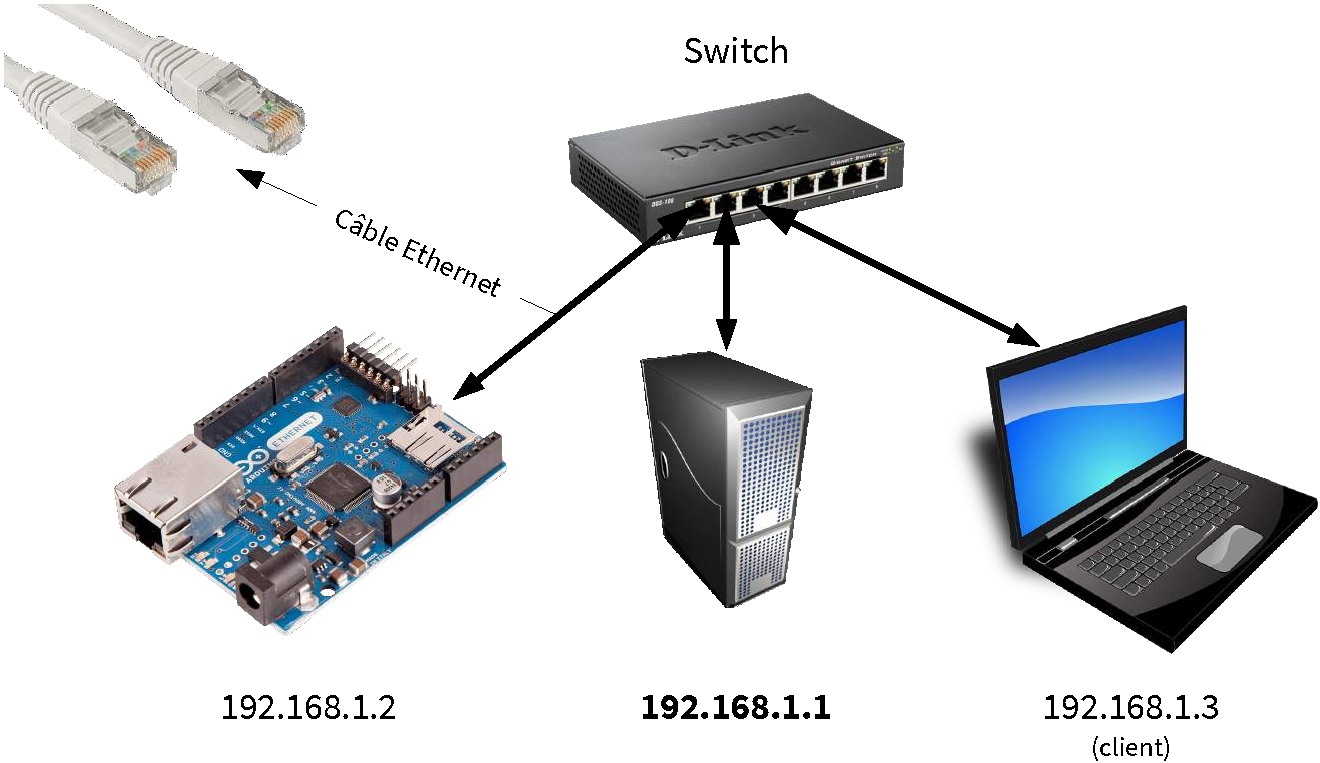
\includegraphics[width=.8\linewidth]{Images/Schema_reseau}
	\caption{Schéma de notre réseau local}
\end{figure}

À l'avenir, si nous utiliserions réellement notre projet, l'Arduino et le serveur n'iraient plus sur un switch mais seraient branchés sur une \emph{box}, le site et la base de données seraient hébergés dans un \emph{data-center} pour que l'utilisateur final y est accès depuis n'importe quelle connexion Internet. Ils n'auront par conséquent plus les mêmes adresses IP.
